% =====================================================================
%  AI-GeSPAD -- VISION AND APPROACH  (upload as a single PDF)
%  UKRI "Enabling AI Adoption Across Science and Engineering" (EPSRC)
%
%  RULES (from call page):  max 4 sides A4 + 1 optional page diagrammatic
%  workplan; single spaced; 11pt Arial or equivalent sans serif;
%  margins >= 2 cm; images/graphs/tables allowed; references allowed
%  (inside the 4 pages).  File name: "<FS number> Vision and Approach".pdf
%
%  Compile:  pdflatex AI-GeSPAD_VisionApproach.tex   (twice)
%  Helvetica (helvet) is metric-equivalent to Arial.  For true Arial use
%  xelatex and uncomment the fontspec lines below.
%
%  \tbc{...} = red text to check / complete; set \showtbcfalse to hide
%  the red highlighting before the final build (text remains!).
% =====================================================================
\documentclass[11pt,a4paper]{article}
\usepackage[a4paper,margin=2cm]{geometry}
\usepackage[T1]{fontenc}
\usepackage[scaled=0.95]{helvet}\renewcommand\familydefault{\sfdefault}
% \usepackage{fontspec}\setmainfont{Arial}   % xelatex alternative
\usepackage[table]{xcolor}
\usepackage{microtype,graphicx,booktabs,tabularx,array,multirow,float,enumitem,caption,tikz}
\definecolor{wpblue}{RGB}{204,224,245}
\definecolor{taskorange}{RGB}{248,196,150}
\definecolor{milestonegreen}{RGB}{200,232,200}
\definecolor{deliverableyellow}{RGB}{255,240,170}
\usetikzlibrary{arrows.meta,positioning,shapes.geometric,fit,calc}
\usepackage[hidelinks]{hyperref}
\usepackage{titlesec,pifont,amsmath,amssymb}
\titleformat{\section}{\normalsize\bfseries\color{blue!45!black}}{}{0pt}{}
\titleformat{\subsection}{\normalsize\bfseries}{}{0pt}{}
\titlespacing*{\section}{0pt}{5pt}{2pt}
\titlespacing*{\subsection}{0pt}{4pt}{1pt}
\setlength{\parindent}{0pt}\setlength{\parskip}{3pt}
\setlist{nosep,leftmargin=1.2em}
\captionsetup{font=small,labelfont=bf,skip=2pt}
\newif\ifshowtbc\showtbctrue
\newcommand{\tbc}[1]{\ifshowtbc\textcolor{red}{#1}\else#1\fi}
\pagestyle{plain}

% ---------------- team macros (edit once) ----------------
\newcommand{\Xin}{Dr Xin Yi}           % domain expert (SPAD device physics)
\newcommand{\Cheng}{Dr Cheng Wang}     % AI expert (safe/trustworthy AI, scenario-based V\&V)

\begin{document}
\begin{center}
{\large\bfseries AI-GeSPAD: AI-enabled design and robustness verification of waveguide-integrated germanium-on-silicon single-photon avalanche diodes}\\[2pt]
\small Vision and Approach \quad|\quad Priority area: Quantum technologies \quad|\quad 12 months from 26 April 2027
\end{center}

% =====================================================================
\section{1. VISION}
% Must cover: quality & importance; potential to advance understanding;
% timeliness; impact (research, society, economy, environment).

\subsection{The domain challenge}
Single-photon detection at the 1550\,nm telecommunications wavelength is a key enabling technology for the quantum internet, photonic quantum computing and long-range quantum-enhanced sensing. These are priority missions in the UK National Quantum Strategy~[1]. The incumbent detectors each carry a major penalty. Superconducting nanowire detectors need cryogenics below about 3\,K. InGaAs/InP SPADs are expensive, are not CMOS-compatible and suffer from afterpulsing~[2]. Germanium-on-silicon (Ge-on-Si) SPADs combine germanium's infrared absorption with silicon's low-noise avalanche multiplication, and they can be made in silicon foundries. Heriot-Watt has led their development, demonstrating planar Ge-on-Si SPADs with record efficiency at 1310\,nm~[3,4], and room-temperature Ge-Si SPAD operation has recently been reported internationally~[5]. \tbc{[Xin: confirm refs 3--5 and the state-of-the-art figures.]}

At 1550\,nm, however, germanium's absorption collapses near its band edge. A normal-incidence device would need a thick Ge layer, which raises dark counts. \textbf{Waveguide integration} decouples the optical absorption length (along the waveguide) from the electrical thickness of the device. This makes it the most credible route to high single-photon detection efficiency (SPDE) at 1550\,nm with a dark count rate (DCR) low enough at the near-room temperatures (230--295\,K) reachable with thermoelectric coolers. Designing such a device is the problem. SPDE and DCR are coupled through mode confinement, absorber geometry, the doping profile that shapes the internal field, avalanche breakdown in Si and tunnelling noise in Ge, and these couplings pull in opposite directions. A high Si field raises the breakdown probability but leaks into Ge and drives tunnelling. A longer absorber raises SPDE but also the thermal dark counts. With more than 10 coupled parameters and TCAD runs of minutes to hours each, one-parameter-at-a-time design explores only a small fraction of the space. A waveguide-coupled Ge-on-Si SPAD with useful 1550\,nm SPDE and low DCR at near-room temperature has not yet been convincingly demonstrated. \tbc{[Xin: confirm wording against the literature.]}

\subsection{The core problem, stated precisely}
Let $\mathbf{x}\in\mathcal{X}\subset\mathbb{R}^{d}$ ($d\approx12$) be the controllable design (waveguide and absorber geometry, multiplication width, charge-sheet dose, excess bias). Let $\boldsymbol{\delta}=(\boldsymbol{\theta},T,\Delta V)\in\Delta$ collect what we cannot control or do not know exactly: the physical model parameters $\boldsymbol{\theta}$ (impact-ionisation coefficients, trap densities, tunnelling parameters), the temperature $T\in[230,295]$\,K and bias drift. TCAD at fidelity $\ell\in\{\mathrm{2D},\mathrm{3D}\}$ (cost $c_\ell$ per run) returns SPDE $\eta(\mathbf{x},\boldsymbol{\delta})$, DCR $D(\mathbf{x},\boldsymbol{\delta})$ and constraints $g_k(\mathbf{x},\boldsymbol{\delta})\le0$ (breakdown-voltage window, Ge field below tunnelling onset, design rules). AI-GeSPAD seeks the \textbf{robust Pareto set}
\begin{equation}
\max_{\mathbf{x}\in\mathcal{X}}\Big(\min_{\boldsymbol{\delta}\in\Delta}\eta(\mathbf{x},\boldsymbol{\delta}),\;-\max_{\boldsymbol{\delta}\in\Delta}\log D(\mathbf{x},\boldsymbol{\delta})\Big)\quad\text{s.t.}\quad\max_{\boldsymbol{\delta}\in\Delta}g_k(\mathbf{x},\boldsymbol{\delta})\le0,\qquad\textstyle\sum_\ell n_\ell c_\ell\le B,
\end{equation}
where $n_\ell$ is the number of runs at fidelity $\ell$ and $B$ the simulation budget. For a target specification $(\eta^*,D^*)$, this reduces to the margin game
\begin{equation}
\max_{\mathbf{x}\in\mathcal{X}}\;\min_{\boldsymbol{\delta}\in\Delta}\;\rho(\mathbf{x},\boldsymbol{\delta}),\qquad \rho=\min\{\eta/\eta^*-1,\;1-D/D^*,\;-g_1,\dots,-g_K\},
\end{equation}
where $\rho\ge0$ means the specification is met. The uncertainty set $\Delta$ is not guessed. It is the 95\% credible region of the posterior $p(\boldsymbol{\theta}\,|\,\text{measured HWU devices})$ combined with the operating ranges, and $P_\mathrm{fail}(\mathbf{x})=\Pr_{\boldsymbol{\delta}}[\rho(\mathbf{x},\boldsymbol{\delta})<0]$ quantifies residual risk. Conventional design solves neither the outer maximisation (too many expensive evaluations) nor the inner minimisation (it checks a few corner cases by hand).

\subsection{Vision: an AI capability the field does not yet have}
AI-GeSPAD will establish a \textbf{robust AI design loop} for semiconductor quantum detectors in which two AI agents play the game in Eq.~(2), and every claim is checked by physics simulation (Fig.~1):
\begin{itemize}
\item \textbf{Designer (outer max).} A \textbf{graph neural network on the TCAD mesh} predicts internal field, absorption and generation maps. Xin's avalanche models then convert these maps into $\eta$, $D$ and $g_k$, and an ensemble of networks gives calibrated uncertainty. Robust multi-objective Bayesian optimisation uses these predictions to choose which design to simulate next and at which fidelity.
\item \textbf{Challenger (inner min).} Using the scenario-based falsification methods \Cheng{} developed to find rare failures of autonomous vehicles~[6,7], an adversarial agent searches $\Delta$ for the physics parameters and operating conditions under which each candidate fails. In effect, it tests whether the AI's conclusion survives what we do not know. Counterexamples become training data and harden the designer's objective.
\item \textbf{Explain.} Field attribution, SHAP and symbolic regression turn the surrogate into \textbf{interpretable design rules} that device physicists can check and reuse.
\end{itemize}
The domain expert (\Xin, SPAD physics) defines the problem, $\Delta$ and the specification. The AI expert (\Cheng, trustworthy AI and simulation-based verification) brings methods proven where trust in AI conclusions is critical.

\begin{figure}[t]\centering
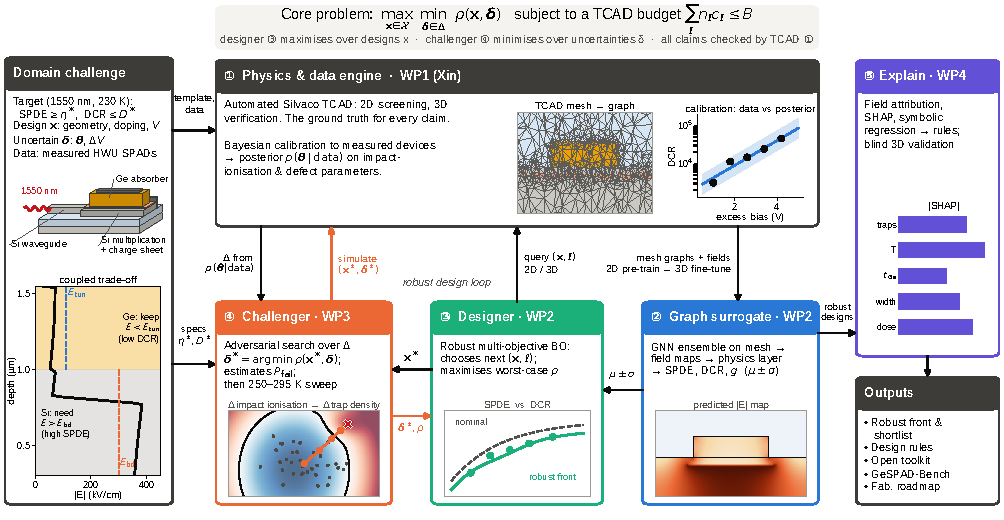
\includegraphics[width=\linewidth]{Fig1_AI-GeSPAD.pdf}
\caption{\textbf{AI-GeSPAD framework.} The physics and data engine \ding{172} (automated TCAD and Bayesian calibration) provides training data and the uncertainty set $\Delta$. The graph surrogate \ding{173} predicts device fields and figures of merit with uncertainty. The designer \ding{174} and the challenger \ding{175} play the robust design game in Eq.~(2), and every candidate and counterexample is re-simulated by \ding{172}. Robust designs are explained and validated blind \ding{176}. Thumbnails are illustrative; the field map and depth profile come from a 2D electrostatic solution of a representative structure.}
\end{figure}

\subsection{Objectives}
\begin{enumerate}[label=\textbf{O\arabic*}]
\item Build a \textbf{calibrated, multi-fidelity simulation pipeline} anchored to measured HWU devices, including the uncertainty set $\Delta$.
\item Develop a \textbf{graph-surrogate designer} that maps the \textbf{robust} SPDE--DCR Pareto front (Eq.~1) at 230\,K.
\item Develop a \textbf{challenger} that verifies the \textbf{robustness of the AI's conclusions} against physics-model and operating uncertainty (Eq.~2).
\item Extract \textbf{interpretable design rules}, release an \textbf{open AI--TCAD toolkit} and benchmark, and set out a \textbf{fabrication roadmap}.
\end{enumerate}

\subsection{Quality, importance and potential to advance understanding}
The scientific prize is new understanding of how photonic confinement, electric-field engineering and avalanche noise interact. Success would give a credible design for a CMOS-compatible telecom single-photon detector that can be integrated on chip. Even a negative result has value: the challenger shows \emph{where} the physics forbids the target.

\subsection{Timeliness}
Ge-on-Si SPAD modelling has matured at HWU~[3,4,8] and internationally~[5]. Graph surrogates and simulation-based falsification are now reliable tools~[6,7]. The EPSRC Integrated Quantum Networks (IQN) Hub, led from HWU, needs integrated telecom detectors~[9]. And the UK is investing in AI for science (AI Opportunities Action Plan, AI for Science Strategy \tbc{[cite]}).

\subsection{Impact}
\textbf{Research:} a reusable \emph{AI-assisted device-research capability} that transfers to other avalanche detectors (Xin's AlInAsSb eSWIR APDs~[10]), lasers and modulators. \textbf{Economy:} CMOS-compatible telecom detectors underpin the UK quantum-networking and LIDAR supply chain,. \textbf{Society and environment:} detectors that need no cryogenics cut the energy and cost of quantum networks, and AI-guided design reduces wasted fabrication runs.

% =====================================================================
\section{2. APPROACH}
% Must cover: effectiveness & appropriateness; feasibility; risks &
% management; methodology; prior work built on; translation of outputs
% into outcomes; research environment.

\subsection{Why this AI approach is appropriate}
Each method answers a feature of Eqs.~(1)--(2), not a wish for novelty. \textbf{(i)} $\eta$ and $D$ are integrals of spatial fields on irregular meshes, with noise dominated by local hot spots. A \textbf{graph neural network on the mesh} matches this structure, and the final step is left to established avalanche physics. \textbf{(ii)} Evaluations are expensive and the budget $B$ is fixed. This calls for \textbf{uncertainty-aware active learning} and 2D-to-3D transfer, with a Gaussian-process baseline as fallback. \textbf{(iii)} The objectives compete, which calls for \textbf{multi-objective} optimisation. \textbf{(iv)} The inner minimum is attained at rare corners of $\Delta$, which calls for \textbf{adversarial falsification and importance sampling} rather than random Monte Carlo~[6,7]. \textbf{(v)} Physicists must trust the answer, so the results must be \textbf{explainable}.

\subsection{Methodology and work packages (Gantt chart on the workplan page)}
\textbf{WP1 -- Calibrated multi-fidelity simulation pipeline (M1--4; lead Xin).} A parameterised device template (waveguide and absorber geometry, multiplication and charge-sheet thickness and doping, guard rings, bias, temperature) drives automated Silvaco runs (Python wrapper, HPC batch) in 2D and in 3D with an optical mode solver. Xin's analytical model gives fast pre-screening. The output metrics are SPDE (absorption $\times$ breakdown probability), DCR (Shockley--Read--Hall, trap-assisted and band-to-band tunnelling) and breakdown voltage. \emph{Calibration:} the impact-ionisation and defect parameters will be fitted by Bayesian calibration to measured current--voltage, SPDE and DCR data from existing HWU Ge-on-Si SPADs~[4,8], with uncertainty carried forward. The posterior defines $\Delta$ and closes the sim-to-real gap.
\emph{Deliverable D1:} automated pipeline and a seed dataset of \tbc{$\sim$1500--3000} mostly 2D simulations, exported as mesh graphs (nodes carry doping, material and field; edges carry mesh connectivity).

\textbf{WP2 -- Graph surrogate and robust designer (M3--9; lead Cheng).} A mesh-based graph neural network (MeshGraphNet-type message passing) is trained to map device structure, bias and temperature to field, absorption and generation maps. A \emph{physics layer} then computes breakdown probability (McIntyre model and Xin's non-uniform-field model~[11]), SPDE and DCR components from those maps. This makes the predictions physically constrained and interpretable. We pre-train on cheap 2D runs and fine-tune on fewer 3D runs, so the multi-fidelity learning happens through transfer. A deep ensemble provides predictive uncertainty. Multi-objective Bayesian optimisation (expected hypervolume improvement) uses the ensemble to select the next simulation and its fidelity. Once the challenger is running, the objective is replaced by its worst case over the counterexamples found so far, approximating the outer maximisation of Eq.~(1). A Gaussian-process surrogate on scalar outputs runs alongside as a baseline and fallback. Design is at 230\,K; robustness up to room temperature is tested in WP3.
\emph{D2:} trained graph surrogate (validated on held-out geometries) and a robust Pareto front with uncertainty bands.

\textbf{WP3 -- Challenger: robustness verification of AI conclusions (M6--10; lead Cheng, with Xin).} Each candidate $\mathbf{x}^*$ is treated as a system under test, as in AV scenario-based testing~[7]. The challenger solves the inner problem $\boldsymbol{\delta}^*=\arg\min_{\boldsymbol{\delta}\in\Delta}\rho(\mathbf{x}^*,\boldsymbol{\delta})$ by Bayesian-optimisation falsification, using the surrogate to search cheaply and TCAD to confirm (about 30--50 2D runs per candidate). It estimates $P_\mathrm{fail}$ by cross-entropy importance sampling. Three sources of failure are targeted: physics-model uncertainty ($\boldsymbol{\theta}$ from the WP1 posterior), operating conditions ($T$ across 230--295\,K, bias drift $\Delta V$) and surrogate error (designs the network rates highly but TCAD rejects). It reports each design's maximum operating temperature. Each counterexample is labelled by its physical mechanism (tunnelling, edge breakdown, loss of efficiency) and fed back to WP2. A final light tolerance check on doping and thickness supports the fabrication roadmap.
\emph{D3:} robustness report per design (worst-case $\rho$, $P_\mathrm{fail}$, counterexamples) and a failure-mechanism catalogue.

\textbf{WP4 -- Explain, validate independently, and plan the legacy (M8--12; joint).} The graph surrogate shows \emph{where} in the device efficiency is gained and noise generated (field and generation maps, node-level attributions). SHAP sensitivity analysis and symbolic regression then give compact design rules, which Xin will check against device physics. \emph{Independent validation:} the shortlisted designs and established reference designs~[3--5] are re-simulated blind at the highest fidelity, using settings the AI never saw. We will release the framework and dataset (Section on data management) and write a fabrication roadmap with partners.
\emph{D4:} design rules, open framework, benchmark, roadmap and follow-on proposal.

\textbf{Success criteria (12 months).} \tbc{[Agree numbers with Xin.]} (a) At least one design with worst-case $\rho\ge0$ over $\Delta$ for $\eta^*=$\,\tbc{X\%}, $D^*=$\,\tbc{Y} counts/s at 230\,K, confirmed by blind 3D TCAD. (b) The designer reaches reference-design performance with at least 5$\times$ fewer high-fidelity runs than a Latin-hypercube baseline. (c) The challenger finds planted failures with at least 5$\times$ fewer runs than random Monte Carlo. (d) At least three validated design rules.

\subsection{Feasibility, prior work and environment}
\Xin{} holds an EPSRC Quantum Technology Career Development Fellowship on next-generation quantum detectors. He has modelled and characterised Ge-on-Si SPADs~[8] and developed avalanche-multiplication models~[11]. He works within Prof.\ Buller's single-photon group at the Institute of Photonics and Quantum Sciences (IPaQS), which has existing Silvaco licences, measured device data and the IQN Hub. \Cheng{} leads the RoboSafe lab, which works on safe and trustworthy AI. His track record includes simulation-based safety assessment under uncertainty~[6], identifying unknown unsafe scenarios~[7] and explainable AI~[12]. These methods transfer directly to WP2--WP4. A full-time, co-supervised PDRA skilled in device simulation and machine learning does most of the work. Computing will use the HWU HPC \tbc{[check: Rocks/Robotarium GPU]}. All methods use mature open-source libraries (PyTorch Geometric, BoTorch, GPyTorch, SHAP, PySR).

\subsection{Risks and management}
\begin{tabularx}{\linewidth}{@{}p{0.31\linewidth}p{0.08\linewidth}X@{}}\toprule
\small\textbf{Risk} & \small\textbf{L/I} & \small\textbf{Mitigation}\\\midrule
\small TCAD too slow for enough samples & \small M/H & \small Multi-fidelity design; 2D runs for most queries; HPC parallel batch; early timing benchmark in M1.\\
\small Simulation does not match real devices & \small M/H & \small Bayesian calibration to measured HWU data (WP1); calibration uncertainty is carried into every prediction.\\
\small Graph surrogate needs more data than available or is overconfident & \small M/M & \small Pre-train on cheap 2D runs, physics layer limits what must be learnt; deep ensembles; GP baseline as fallback; adversarial falsification (WP3); blind high-fidelity validation (WP4).\\
\small Target not physically achievable & \small L/M & \small Falsification shows the physical limits, a publishable roadmap result; the maximum operating temperature per design gives a graded fallback target.\\
\small PDRA recruitment delay & \small M/M & \small Advertise on award; named candidates \tbc{[if any]}; leads cover M1--2.\\\bottomrule
\end{tabularx}

\subsection{From outputs to outcomes, and legacy}
\textbf{Within 12 months:} a design shortlist, rules, an open framework and a dataset. \textbf{Next 1--3 years:} fabrication of the top designs through IQN Hub and partner cleanrooms \tbc{[e.g. Glasgow JWNC / CORNERSTONE -- partner letters]}, plus a follow-on proposal (EPSRC standard or IQN Hub flexible fund). \textbf{Legacy:} the framework is device-agnostic. It will be reused in Xin's eSWIR APD programme and offered to the UK quantum-detector community through the annual programme workshop, the IQN Hub and a hands-on tutorial. It also creates a lasting IPaQS--Robotics collaboration.

% ---------------- References (count within 4 pages) ----------------
\vspace{2pt}\hrule\vspace{2pt}
{\scriptsize \textbf{References} \tbc{[verify all]}
[1] DSIT, \emph{National Quantum Strategy} (2023); Quantum Missions (2023).
[2] Saalbach, Fleming, Yi, Buller, \emph{Adv. Phys. X} (2026).
[3] Vines \emph{et al.}, \emph{Nat. Commun.} 10, 1086 (2019).
[4] Mirza \emph{et al.}, \tbc{Ge-on-Si SPAD 1310/1550 nm paper, HWU/Glasgow}.
[5] Na \emph{et al.}, \emph{Nature} 627, 295 (2024).
[6] Wang \& Winner, \emph{IEEE T-IV} (2020).
[7] Wang \emph{et al.}, \emph{Accid. Anal. Prev.} (2024), runtime unknown unsafe scenario identification for SOTIF.
[8] Muir \emph{et al.}, \emph{IEEE T-ED} (2025).
[9] EPSRC Integrated Quantum Networks Hub (2024).
[10] Jin \emph{et al.}, \emph{ACS Photonics} (2026).
[11] Jin, Yi \emph{et al.}, \emph{AIP Adv.} (2026).
[12] Kuznietsov, Gyevnar, Wang \emph{et al.}, \emph{IEEE T-ITS} (2024).\par}

% ============================================================
%% ADDITIONAL PAGE: DIAGRAMMATIC WORKPLAN (max 1 page A4)
% ============================================================
\clearpage
\begin{table}[H]
\vspace*{-\intextsep}
\centering
{\large\bfseries AI-GeSPAD: 12-month workplan (start 26 April 2027)}\\[1pt]
{\itshape (Xin Yi leads WP1, Cheng Wang leads WP2--WP3, WP4 is joint; the PDRA contributes to all WPs)}\\[4pt]
\setlength{\tabcolsep}{2pt}
\begin{tabularx}{\textwidth}{|p{2.45cm}|*{12}{>{\centering\arraybackslash}X|}}
\hline
\textbf{Quarter} & \multicolumn{3}{c|}{\textbf{Q1}} & \multicolumn{3}{c|}{\textbf{Q2}} & \multicolumn{3}{c|}{\textbf{Q3}} & \multicolumn{3}{c|}{\textbf{Q4}} \\
\cline{2-13}
\textbf{Month} & M1 & M2 & M3 & M4 & M5 & M6 & M7 & M8 & M9 & M10 & M11 & M12 \\
\hline
\rowcolor{wpblue}
\multicolumn{13}{|l|}{\textbf{WP1: Physics \& data engine (Xin Yi, PDRA)}}\\
\hline
T1.1 & \cellcolor{taskorange} & \cellcolor{taskorange} &  &  &  &  &  &  &  &  &  &  \\
\hline
T1.2 &  & \cellcolor{taskorange} & \cellcolor{taskorange} & \cellcolor{taskorange} &  &  &  &  &  &  &  &  \\
\hline
\rowcolor{wpblue}
\multicolumn{13}{|l|}{\textbf{WP2: Graph surrogate and robust designer (Cheng Wang, PDRA)}}\\
\hline
T2.1 &  &  & \cellcolor{taskorange} & \cellcolor{taskorange} & \cellcolor{taskorange} & \cellcolor{taskorange} &  &  &  &  &  &  \\
\hline
T2.2 &  &  &  &  & \cellcolor{taskorange} & \cellcolor{taskorange} & \cellcolor{taskorange} & \cellcolor{taskorange} & \cellcolor{taskorange} &  &  &  \\
\hline
\rowcolor{wpblue}
\multicolumn{13}{|l|}{\textbf{WP3: Challenger -- robustness verification of AI conclusions (Cheng Wang, Xin Yi, PDRA)}}\\
\hline
T3.1 &  &  &  &  &  & \cellcolor{taskorange} & \cellcolor{taskorange} & \cellcolor{taskorange} & \cellcolor{taskorange} &  &  &  \\
\hline
T3.2 &  &  &  &  &  &  &  &  & \cellcolor{taskorange} & \cellcolor{taskorange} &  &  \\
\hline
\rowcolor{wpblue}
\multicolumn{13}{|l|}{\textbf{WP4: Explain, validate and legacy (Xin Yi, Cheng Wang, PDRA)}}\\
\hline
T4.1 &  &  &  &  &  &  &  & \cellcolor{taskorange} & \cellcolor{taskorange} & \cellcolor{taskorange} & \cellcolor{taskorange} &  \\
\hline
T4.2 &  &  &  &  &  &  &  &  &  & \cellcolor{taskorange} & \cellcolor{taskorange} &  \\
\hline
T4.3 &  &  &  &  &  &  &  &  &  &  & \cellcolor{taskorange} & \cellcolor{taskorange} \\
\hline
\rowcolor{milestonegreen}
Milestones: &  &  &  & MS1 &  & MS2 &  &  & MS3 & MS4 &  & MS5 \\
\hline
\rowcolor{deliverableyellow}
Deliverables: &  &  &  & D1 &  &  &  &  & D2 & D3 &  & D4 \\
\hline
\end{tabularx}

\vspace{3pt}
% ===== TASKS =====
\noindent\textbf{Tasks:}\\[2pt]
\begin{tabularx}{\textwidth}{|>{\columncolor{taskorange}}p{2.3cm}|X|}
\hline
T1.1: & Parameterised device template and automated 2D/3D Silvaco TCAD pipeline on HPC \\
\hline
T1.2: & Bayesian calibration to measured HWU Ge-on-Si SPADs; posterior $p(\boldsymbol{\theta}\,|\,\text{data})$ defines the uncertainty set $\Delta$ \\
\hline
T2.1: & Graph surrogate on the TCAD mesh: 2D pre-training, 3D fine-tuning, ensemble uncertainty; comparison with GP baseline \\
\hline
T2.2: & Robust multi-objective Bayesian optimisation of SPDE and DCR at 230\,K \\
\hline
T3.1: & Adversarial falsification over $\Delta$ (physics parameters, $T$ across 230--295\,K, $\Delta V$, surrogate error) and importance-sampling estimate of $P_\mathrm{fail}$ \\
\hline
T3.2: & Counterexample feedback to the designer; robust ranking and failure-mechanism labelling \\
\hline
T4.1: & Field attribution, SHAP and symbolic regression to extract physical design rules \\
\hline
T4.2: & Blind high-fidelity 3D validation of shortlisted and reference designs \\
\hline
T4.3: & Open release (toolkit, GeSPAD-Bench dataset), fabrication roadmap and follow-on proposal \\
\hline
\end{tabularx}

\vspace{3pt}
% ===== MILESTONES =====
\noindent\textbf{Milestones:}\\[2pt]
\begin{tabularx}{\textwidth}{|>{\columncolor{milestonegreen}}p{2.3cm}|X|}
\hline
MS1 (M4): & Calibrated simulation pipeline running; uncertainty set $\Delta$ defined \\
\hline
MS2 (M6): & Graph surrogate validated on held-out geometries; surrogate choice for the design loop confirmed; partner review \\
\hline
MS3 (M9): & Robust SPDE--DCR Pareto front mapped at 230\,K \\
\hline
MS4 (M10): & Shortlisted designs verified by the challenger (worst-case $\rho$, $P_\mathrm{fail}$, maximum operating temperature) \\
\hline
MS5 (M12): & Design rules validated blind; open toolkit and dataset released; final partner review \\
\hline
\end{tabularx}

\vspace{3pt}
% ===== DELIVERABLES =====
\noindent\textbf{Deliverables:}\\[2pt]
\begin{tabularx}{\textwidth}{|>{\columncolor{deliverableyellow}}p{2.3cm}|X|}
\hline
D1 (M4): & Automated, calibrated TCAD pipeline and seed simulation dataset (internal release) \\
\hline
D2 (M9): & Trained graph surrogate and robust Pareto front with uncertainty bands (a journal paper) \\
\hline
D3 (M10): & Robustness report per design and failure-mechanism catalogue (a conference paper) \\
\hline
D4 (M12): & Design rules, open AI--TCAD toolkit and GeSPAD-Bench dataset, fabrication roadmap; results presented at the programme workshop and a community tutorial \\
\hline
\end{tabularx}
\caption{Additional page for the diagrammatic workplan.}
\label{tab:workplan}
\end{table}

\end{document}
